\newcommand\nd{15mm}
	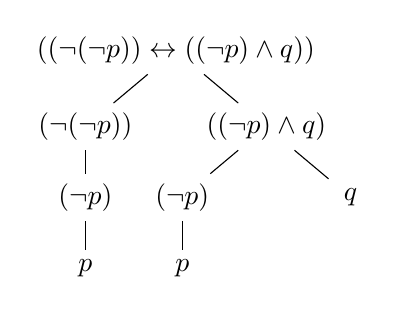
\begin{tikzpicture}[
			vertex/.style={draw=none,rectangle,minimum width=7mm},
			% node distance=10mm,
			scale=1, every node/.style={scale=1}
		]
		\node [vertex] (v0) {$((\neg(\neg p))\leftrightarrow ((\neg p)\wedge q))$};
		% \node [vertex,label=above:{$-1$}] (v0) {$H$};
		\node [vertex] (v1) at ([shift=({220:1*\nd})]v0)  {$(\neg(\neg p))$};
		\node [vertex] (v2) at ([shift=({320:1*\nd})]v0)  {$((\neg p)\wedge q)$};

		\node [vertex] (v3) at ([shift=({270:0.6*\nd})]v1)  {$(\neg p)$};
		\node [vertex] (v4) at ([shift=({270:0.6*\nd})]v3)  {$p$};

		\node [vertex] (v5) at ([shift=({220:0.93*\nd})]v2)  {$(\neg p)$};
		\node [vertex] (v6) at ([shift=({320:0.93*\nd})]v2)  {$q$};


		\node [vertex] (v7) at ([shift=({270:0.6*\nd})]v5)  {$p$};

		
		\draw[] (v0)--(v1);
		\draw[] (v0)--(v2);
		\draw[] (v1)--(v3);
		\draw[] (v3)--(v4);
		\draw[] (v2)--(v5);
		\draw[] (v2)--(v6);
		\draw[] (v5)--(v7);
	\end{tikzpicture}